\documentclass[conference]{IEEEtran}

\usepackage{amsmath,amssymb}
\usepackage{booktabs}
\usepackage{balance}
\usepackage{cite}
\usepackage{graphicx}
\usepackage{algorithmic}
\usepackage{microtype}
\usepackage[hidelinks]{hyperref}
\newcommand{\method}{SC-ICDM}
\newcommand{\vect}[1]{\boldsymbol{#1}}
\newcommand{\norm}[1]{\left\lVert#1\right\rVert}
\newcommand{\pos}[1]{\left[#1\right]_{+}}
\hyphenation{com-mu-ni-ca-tions}

\begin{document}
\title{Self-Calibrated Diffusion Interference Cancellation\\
under Nonstationary Interference}
\author{
\IEEEauthorblockN{Author Name(s)}
\IEEEauthorblockA{Department or Institution\\
City, Country\\
email@domain.com}
}
\maketitle

\begin{abstract}
Diffusion interference cancellation relies on an interference scale that is
often selected from the true signal-to-interference-plus-noise ratio (SINR).
An unknown scale, particularly one that varies within a frame, creates a
mismatch between the received signal and the likelihood used for
reconstruction. This paper proposes a self-calibrated interference
cancellation diffusion model (SC-ICDM) for wireless image transmission.
The receiver initializes blockwise interference powers from received energy,
then alternates diffusion reconstruction with nonnegative least-squares
amplitude updates. The updates also adapt the local likelihood guidance and
reuse existing denoiser outputs without retraining. An exploratory evaluation
over 200 image pairs, three interference profiles, and six SINR values shows
a mean PSNR gain of 0.599~dB over one-shot blockwise calibration, with a
95\% image-pair-cluster bootstrap interval of 0.551--0.648~dB.
The gain reaches 1.478~dB relative to the true-global-SINR reference.
However, updates degrade reconstruction under severe burst interference,
and direct decoding remains preferable at the weakest tested interference.
These results establish the value of local receiver calibration in the
tested setting while identifying its operating limits.
\end{abstract}

\begin{IEEEkeywords}
semantic communications, interference cancellation, diffusion models,
SINR estimation, nonstationary interference
\end{IEEEkeywords}

\section{Introduction}

A wireless image receiver must reconstruct its source from channel
observations that can contain both noise and structured interference.
Deep joint source-channel coding (JSCC) learns this mapping through an
encoder and decoder trained across the channel~\cite{bourtsoulatze2019deep}.
Semantic communication methods can additionally shape the representation
to preserve information needed for downstream tasks, as demonstrated by
contrastive learning for image transmission~\cite{tang2023contrastive}.
At the receiver, however, an interfering transmission need not resemble
the Gaussian perturbations used during training. Its structure and power
then become relevant to reconstruction.

Learned interference cancellation offers two approaches to this problem.
A direct separation network maps the received mixture to the desired
waveform; for example, Fourier-convolution networks have been studied for
blind co-channel cancellation~\cite{naseri2024blind}. A generative receiver
instead uses learned priors to constrain the components that explain the
observation. Channel denoising diffusion models (CDDMs) apply such a prior
to suppress channel noise~\cite{wu2024cddm}. The interference cancellation
diffusion model (ICDM) extends this principle by coupling separate desired
signal and interference priors through a shared likelihood~\cite{wu2026icdm}.
The latter approach is attractive when pretrained priors are available
and adaptation can be confined to inference.

The ICDM implementation considered here selects its interference amplitude
and guidance coefficients from the true frame-level SINR. Two difficulties
arise when that information is unavailable. First, the receiver must infer
the scale from the mixture itself. Second, even an accurate frame average
cannot describe a transmission in which interference power changes across
blocks. A global energy estimate addresses the missing side information,
but discards these local differences. Independent block estimates preserve
them at the cost of greater sensitivity to local signal energy and
finite-sample cross terms.

The diffusion trajectory provides another source of information. As
reconstruction proceeds, the receiver obtains estimates of both components
of the mixture. Given those estimates, fitting a nonnegative interference
amplitude requires only a scalar least-squares problem per block. The fitted
amplitudes can then be returned to the likelihood correction. This
alternation uses information already computed by the receiver and keeps
the pretrained networks fixed. Joint estimation of signals and unknown
forward parameters has precedents in blind diffusion inverse problems,
including GibbsDDRM~\cite{murata2023gibbsddrm}; the question here is whether
a simple blockwise point update is useful within an ICDM communication
receiver.

We propose \method{}, a receiver that initializes its local powers from
received energy and refines them during reverse diffusion. Our contributions
are threefold:
\begin{itemize}
    \item A SINR-blind formulation of ICDM with blockwise interference
    amplitudes and receiver information specified explicitly.
    \item A closed-form calibration update that adapts both the interference
    scale and local guidance without additional denoiser evaluations.
    \item A matched evaluation separating global estimation, local
    initialization, and iterative refinement, including the regimes where
    refinement or cancellation reduces reconstruction quality.
\end{itemize}

Across the tested profiles, \method{} improves mean PSNR by 0.599~dB over
one-shot blockwise calibration. The result concerns reconstruction: the
estimated powers do not consistently approach the physical powers.
Section~II defines the signal model and receiver assumptions.
Section~III develops the calibration procedure, and Section~IV evaluates
its gains and limitations before Section~V concludes the paper.

\section{System Model and Problem Formulation}

\subsection{Image Transmission with Blockwise Interference}

Let $\vect{s}$ denote the source image and let
$\vect{x}=f_{\mathrm{enc}}(\vect{s})\in\mathbb{C}^{N}$ be its transmitted
JSCC representation, normalized to $\norm{\vect{x}}_2^2/N=1$.
An independent interference image produces a latent vector
$\vect{z}\in\mathbb{C}^{N}$ with the same framewise normalization.
A fixed partition $\{\mathcal{B}_b\}_{b=1}^{B}$ divides the transmitted
symbol order into blocks of length $L_b=|\mathcal{B}_b|$.
We consider the AWGN observation
\begin{equation}
    \vect{y}_b=\vect{x}_b+a_b\vect{z}_b+\vect{n}_b,\qquad
    \vect{n}_b\sim\mathcal{CN}(\vect{0},N_0\vect{I}),
    \label{eq:system}
\end{equation}
where $a_b\geq0$ is constant within block $b$ but unknown to the receiver.
One amplitude multiplies both components of each complex symbol.
The nominal interference power and nominal SINR are
\begin{equation}
    \bar p=\frac{1}{N}\sum_{b=1}^{B}L_ba_b^2,\qquad
    \gamma=-10\log_{10}(\bar p+N_0).
    \label{eq:nominal}
\end{equation}
Here $a_b^2$ is a model coefficient. The realized interference energy in
block $b$ is $a_b^2\norm{\vect{z}_b}_2^2/L_b$, which need not equal
$a_b^2$ because normalization is applied to the complete frame.

The receiver returns a desired latent estimate $\widehat{\vect{x}}$ and
reconstructs the image as
$\widehat{\vect{s}}=f_{\mathrm{dec}}(\widehat{\vect{x}})$.
We hold the encoder, decoder, and diffusion priors fixed so that changes
in reconstruction can be attributed to the receiver procedure.

\subsection{Available Information and Calibration Objective}

The receiver observes $\vect{y}$ and knows $N_0$, the block partition,
and the pretrained desired and interference priors. It has no access to
the clean latents, block amplitudes, profile label, or true SINR.
Thus, \emph{SINR-blind} refers specifically to the missing interference-power
information; the noise level and interference family remain known.

For fixed $\vect{a}=(a_1,\ldots,a_B)$, the Gaussian model gives
\begin{equation}
 -\log p(\vect{y}\mid\vect{x},\vect{z},\vect{a})
 =\frac{1}{N_0}\sum_b
 \norm{\vect{y}_b-\vect{x}_b-a_b\vect{z}_b}_2^2+C,
 \label{eq:likelihood}
\end{equation}
where $C$ is independent of the latent vectors and amplitudes.
ICDM uses its two priors to guide recovery of these latent vectors.
Our task is to supply useful local amplitudes throughout that recovery
when $\vect{a}$ is unknown. The objective is image reconstruction; accurate
physical power estimation is a separate property to be tested.

\section{Self-Calibrated Diffusion Receiver}

\subsection{Initialization from Received Energy}

Under unit expected signal and interference power and vanishing cross
moments, the expected received energy in a block is $1+a_b^2+N_0$.
This motivates the initialization
\begin{equation}
    \widehat p_b^{(0)}
    =\pos{\norm{\vect{y}_b}_2^2/L_b-1-N_0},\qquad
    \widehat a_b^{(0)}=\sqrt{\widehat p_b^{(0)}},
    \label{eq:init}
\end{equation}
where $[u]_+=\max(u,0)$. Using the full frame in~\eqref{eq:init}
gives a global estimate; using individual blocks retains local variation.
The latter is an energy proxy, since framewise normalization does not
enforce unit power in each block. Local latent energy, noise fluctuations,
and signal--interference cross terms all contribute to its error.

For any current power estimate, the corresponding local SINR is
\begin{equation}
    \widehat\gamma_b=-10\log_{10}(\widehat p_b+N_0).
    \label{eq:local_sinr}
\end{equation}
We obtain the guidance coefficients $(\lambda_b,\beta_b)$ by linear
interpolation of the fixed ICDM lookup table. At the AWGN SINR knots
$(-7,-4,0,4,7,10,20)$~dB, the respective coefficient sequences are
$(0.3,1,1.4,3,4.5,5.5,3)$ and $(0.1,0.7,1,1,1,0.5,2)$.
Values outside the range use the nearest endpoint. These inherited
coefficients are not optimized on the reported image pairs.

\subsection{Amplitude Refinement from Denoised Estimates}

Let $\alpha_t$ and $\sigma_t$ denote the forward diffusion signal and
noise coefficients. At a reverse step, the two frozen noise predictors
provide clean-point estimates
\begin{equation}
\begin{split}
 \widehat{\vect{x}}_0^{(t)}
 &=\frac{\vect{x}_t-\sigma_t
       \vect{\epsilon}_{\theta_x}(\vect{x}_t,t)}{\alpha_t},\\
 \widehat{\vect{z}}_0^{(t)}
 &=\frac{\vect{z}_t-\sigma_t
       \vect{\epsilon}_{\theta_z}(\vect{z}_t,t)}{\alpha_t}.
\end{split}
\label{eq:points}
\end{equation}
Before fitting amplitudes, we normalize each complete-frame estimate:
\begin{equation}
 \Pi(\vect{u})=
 \frac{\vect{u}}{\sqrt{\max(\norm{\vect{u}}_2^2/N,\epsilon_{\rm mach})}},
 \quad
 \widetilde{\vect{x}}_0^{(t)}=\Pi(\widehat{\vect{x}}_0^{(t)}),
 \label{eq:project}
\end{equation}
and similarly for $\widetilde{\vect{z}}_0^{(t)}$.
This projection imposes the transmitter power convention on the estimated
components. It is applied over the frame rather than separately within
each block, allowing local latent-energy variation to remain.

For fixed projected components, the likelihood in~\eqref{eq:likelihood}
separates into independent scalar problems:
\begin{equation}
 \min_{a\geq0}\ 
 \norm{\vect{y}_b-\widetilde{\vect{x}}_{0,b}^{(t)}
                  -a\widetilde{\vect{z}}_{0,b}^{(t)}}_2^2.
 \label{eq:ls}
\end{equation}
Define
$h_b=\norm{\widetilde{\vect{z}}_{0,b}^{(t)}}_2^2$ and
$c_b=\operatorname{Re}\{
(\widetilde{\vect{z}}_{0,b}^{(t)})^H
(\vect{y}_b-\widetilde{\vect{x}}_{0,b}^{(t)})\}$.
The objective is $h_ba^2-2c_ba+\text{const}$.
Differentiating and imposing nonnegativity gives the implemented update
\begin{equation}
 \widehat a_b^{\rm new}=
 \begin{cases}
    [c_b/h_b]_+, & h_b>L_b\epsilon_{\rm mach},\\
    \widehat a_b^{\rm old}, & \text{otherwise}.
 \end{cases}
 \label{eq:amplitude}
\end{equation}
The fallback prevents division by a numerically empty estimate.
There is no ridge penalty or amplitude cap in the evaluated update.

Calibration begins when $\alpha_t\geq0.5$; earlier steps retain the energy
initialization. Because~\eqref{eq:points} divides by $\alpha_t$, this delay
avoids fitting from clean-point estimates at the noisiest end of the
trajectory. It is a fixed activation rule, not an estimate of whether a
particular block is reliable. The evaluated 40-step, order-3 UniPC schedule
performs 21 calibration updates.

\subsection{Feedback into the ICDM Sampler}

After each amplitude update, the receiver sets
$\widehat p_b=(\widehat a_b^{\rm new})^2$ and recomputes the local guidance
coefficients using~\eqref{eq:local_sinr}. To make the role of calibration
explicit, the AWGN likelihood correction inherited from ICDM can be
written, at the states entering that correction, as
\begin{equation}
 \vect{r}_{t,b}=\vect{y}_b/\zeta_t-\vect{x}_{t,b}
                  -\widehat a_b\vect{z}_{t,b},\qquad
 \zeta_t=(2-\alpha_t^2)^{-1},
 \label{eq:residual}
\end{equation}
\begin{equation}
\begin{split}
 \vect{\epsilon}^{\,g}_{x,b}
    &=\vect{\epsilon}_{x,b}-\zeta_t^2\lambda_b\vect{r}_{t,b},\\
 \vect{\epsilon}^{\,g}_{z,b}
    &=\vect{\epsilon}_{z,b}
        -\zeta_t^2\beta_b\widehat a_b\vect{r}_{t,b}.
\end{split}
\label{eq:guidance}
\end{equation}
Here $\vect{\epsilon}_{x,b}$ and $\vect{\epsilon}_{z,b}$ are the noise
predictions used by the sampler. The block amplitudes and coefficients
are broadcast over their associated symbols. The numerical integration
and likelihood correction otherwise follow the retained ICDM implementation.

Equations~\eqref{eq:amplitude}--\eqref{eq:guidance} form the feedback loop:
the current reconstruction determines the next amplitude, and that
amplitude changes the subsequent reconstruction. The update changes both
the mixture scale and the guidance strength. Accordingly, the experiments
evaluate their combined effect; they do not isolate either factor.

The complete procedure is summarized below. It reuses the two noise
predictions already required at each eligible corrector step.

\begin{quote}
\textbf{SC-ICDM inference}
\begin{algorithmic}[1]
\STATE Initialize $\widehat p_b,\widehat a_b$ by~\eqref{eq:init}.
\STATE Initialize the two diffusion states as in ICDM.
\FOR{each reverse sampling step}
    \STATE Advance the two UniPC predictors.
    \IF{a corrector evaluation is available}
        \STATE Evaluate the two frozen noise predictors.
        \IF{$\alpha_t\geq0.5$}
            \STATE Form and project the estimates in~\eqref{eq:points}--\eqref{eq:project}.
            \STATE Update all amplitudes by~\eqref{eq:amplitude}.
        \ENDIF
        \STATE Apply the UniPC corrector and local guidance
        using the current amplitudes and coefficients.
    \ENDIF
\ENDFOR
\STATE Normalize the recovered desired latent and decode.
\end{algorithmic}
\end{quote}

Each calibration pass requires linear work in $N$ for normalization,
inner products, and blockwise reductions, plus $O(B)$ coefficient
interpolation. It adds no denoiser call or trainable parameter.
The least-squares step minimizes~\eqref{eq:ls} for fixed point estimates,
but those estimates change during diffusion. Consequently, this local
minimization does not establish monotonic improvement of image quality or
convergence of a joint posterior objective.

\section{Simulation Results}

\subsection{Experimental Settings}

We evaluate 200 CelebA desired images paired with CIFAR-10 interference
images, reconstructing the desired images at $128\times128$ resolution.
All receivers use the same frozen SwinJSCC encoder and decoder
\cite{yang2025swinjscc}, interference encoder, and two DiT diffusion priors.
The latent bottleneck has eight channels. Noise SNR is fixed at 20~dB;
nominal SINR takes values in $\{-7,-4,0,4,7,10\}$~dB.
Each pair is evaluated under three channel seeds and three interference
profiles, giving 10,800 reconstructions per receiver.

Blocks contain 64 complex symbols. The stationary profile has equal block
powers; alternating and burst profiles repeat power multipliers
$(0.25,1.75)$ and $(0,2)$, respectively. The multipliers are normalized
to preserve the nominal frame average. These profiles test the effect
of local power variation while keeping the nominal SINR fixed.
Their boundaries coincide with the receiver partition.

We compare the following receivers:
\begin{itemize}
    \item \emph{Direct}: JSCC decoding without diffusion cancellation.
    \item \emph{Global-SINR} (A0): ICDM with true global SINR and the
    original amplitude convention.
    \item \emph{Global-blind} (A2): one received-energy estimate for
    the complete frame.
    \item \emph{Block-blind} (A3): blockwise initialization
    from~\eqref{eq:init}, held fixed throughout diffusion.
    \item \emph{SC-ICDM} (A4): the proposed alternating calibration.
\end{itemize}
Global-SINR knows the nominal frame average but not the local profile,
so it is a reference rather than an upper bound. An additional control
(A1) corrects its amplitude convention while keeping the true SINR.
Every diffusion receiver uses 40 order-3 UniPC steps with the same number
of network evaluations.

Comparisons are paired by desired image, interference image, channel seed,
and diffusion initialization. PSNR is computed per reconstruction before
averaging. For \method{} contrasts, we report 95\% percentile bootstrap
intervals from 10,000 resamples of the 200 image-pair clusters, retaining
all seeds and operating conditions within each selected cluster.
The image pairs were inspected during method development. The intervals
therefore describe exploratory results and are not adjusted for multiple
comparisons.

\begin{figure*}[t]
\centering
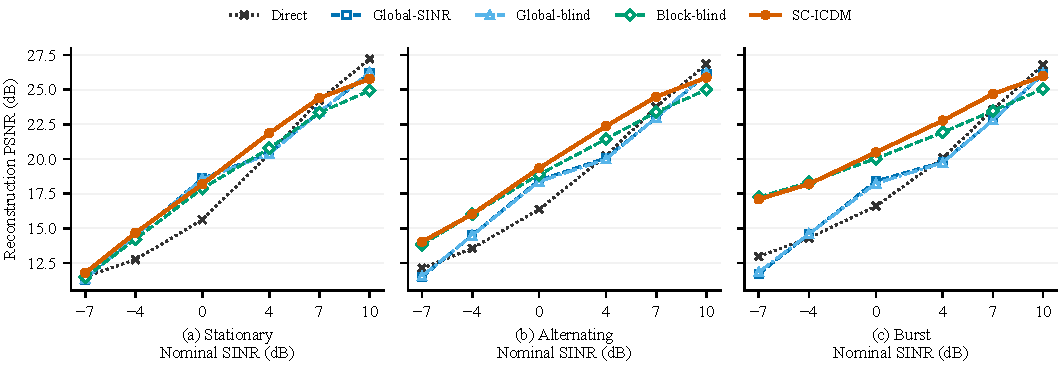
\includegraphics[width=\textwidth]{figures/fig_psnr.pdf}
\caption{Reconstruction PSNR versus nominal SINR under the three power
profiles. Each point averages 200 image pairs and three channel seeds.
Global-SINR and Global-blind nearly overlap. The direct-decoding curves
show why an improvement over another cancellation receiver need not imply
an improvement over omitting cancellation.}
\label{fig:psnr}
\end{figure*}

\subsection{Global and Blockwise Calibration}

Table~\ref{tab:psnr} separates the effect of estimating the global power
from that of retaining local variation. Global-blind differs from
Global-SINR by only $-0.005$, $-0.008$, and $-0.005$~dB for stationary,
alternating, and burst interference, respectively. Thus, a blind energy
estimate closely reproduces the mean reconstruction quality of the
global reference in this experiment. These small descriptive differences
do not by themselves establish statistical equivalence.
Fig.~\ref{fig:psnr} gives the corresponding PSNR curves, retaining the
individual SINR values that are averaged in the table.

\begin{table}[t]
\caption{Mean PSNR (dB) over 200 image pairs, three seeds, and six SINR values.
The final column also averages over the three profiles.}
\label{tab:psnr}
\centering
\setlength{\tabcolsep}{3.4pt}
\begin{tabular}{lrrrr}
\toprule
Receiver & Stationary & Alternating & Burst & All\\
\midrule
Direct       & 18.616 & 18.811 & 19.047 & 18.825\\
Global-SINR  & 19.058 & 18.939 & 18.903 & 18.967\\
Global-blind & 19.053 & 18.931 & 18.898 & 18.961\\
Block-blind  & 18.767 & 19.758 & 21.012 & 19.845\\
\method{}    & \textbf{19.446} & \textbf{20.352}
             & \textbf{21.535} & \textbf{20.444}\\
\bottomrule
\end{tabular}
\end{table}

Block-blind gains 0.819~dB and 2.108~dB over Global-SINR in the
alternating and burst cases. It loses 0.292~dB under stationary
interference, where separate blocks contain no additional power-profile
information. The pattern is consistent with the trade-off in
\eqref{eq:init}: shorter averaging windows retain local changes but also
retain local fluctuations. Correcting only the original amplitude
convention changes mean PSNR by 0.007--0.010~dB across profiles, far
less than the nonstationary blockwise gains.

\subsection{Benefit and Limits of Iterative Refinement}

\method{} improves Block-blind by 0.599~dB overall, with a 95\% cluster
interval of 0.551--0.648~dB. The profile-specific gains are
0.680~dB for stationary interference, 0.594~dB for alternating
interference, and 0.523~dB for burst interference, with respective
intervals of 0.629--0.729, 0.540--0.649, and 0.469--0.578~dB.
The proposed receiver exceeds Block-blind in 79.1\% of matched trials.
Relative to Global-SINR, the overall gain is 1.478~dB
(1.392--1.563~dB).

Fig.~\ref{fig:gain} shows how refinement depends on the operating point.
Averaging across profiles, the gain over Block-blind increases from
0.118~dB at $-7$~dB SINR to 1.122~dB at 7~dB SINR.
The burst profile is the exception at strong interference: refinement
loses 0.174~dB at $-7$~dB SINR and 0.109~dB at $-4$~dB SINR.
The corresponding intervals for the signed differences are
$[-0.224,-0.126]$ and $[-0.197,-0.025]$~dB.
For alternating interference at $-4$~dB, the difference is just
0.001~dB with interval $[-0.092,0.092]$~dB.
An average improvement therefore does not justify updating every
interference realization.

\begin{figure}[t]
\centering
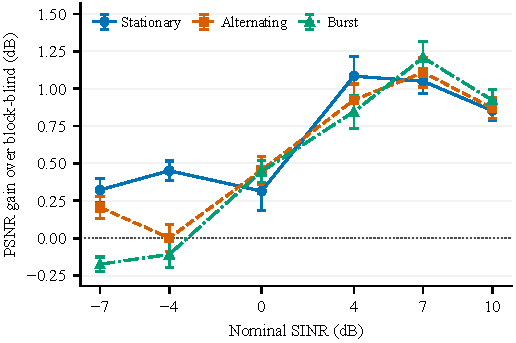
\includegraphics[width=\columnwidth]{figures/fig_calibration.pdf}
\caption{Paired PSNR gain of SC-ICDM over Block-blind. Bars show exploratory
95\% image-pair-cluster bootstrap intervals. Negative values at low SINR
under burst interference identify operating points where refinement hurts.}
\label{fig:gain}
\end{figure}

The comparison with Direct answers a different question: whether
cancellation itself is beneficial. At 10~dB SINR, \method{} gains
0.882~dB over Block-blind but is still 1.070~dB below Direct
(interval $[-1.270,-0.867]$~dB). At this operating point, improved
calibration does not remove the disadvantage of invoking the diffusion
receiver. A practical extension is to choose between direct decoding and
cancellation from receiver-observable evidence; no such selection rule
is evaluated here.

\subsection{Power Estimates and Computational Cost}

The final amplitudes should not be interpreted as consistently improved
physical-power estimates. Although \method{} improves reconstruction in
79.1\% of trials, its block-power RMSE improves over initialization in only
28.3\%. At SINR values of 0, 4, and 10~dB, median final power estimates
are 0.234, 0.024, and 0.004, compared with nominal frame powers of
0.990, 0.388, and 0.090. Fourteen trials contain an estimated block
power above 100; the maximum is 93,186.656. The numerical fallback in
\eqref{eq:amplitude} therefore does not prevent all large estimates.

These diagnostics support interpreting the update as a reconstruction
calibration mechanism. They do not support a claim of accurate power
recovery. Small interference-estimate energy can amplify the ratio in
\eqref{eq:amplitude}, but the recorded outputs do not establish which
mechanism causes the observed outliers or the severe-burst losses.
Separate scale and guidance ablations would also be needed to determine
which part of the feedback contributes most to the PSNR gain.

\balance
Measured receiver time is 0.323~s per image for Block-blind and 0.347~s
for \method{} on an RTX~4090 with batch size four. Timing includes
calibration, sampling, output normalization, and decoding, with GPU
synchronization; encoding, data loading, and channel generation are excluded.
The measurements come from separate runs and should be read as descriptive
timings, not as a controlled estimate of overhead or batch-one latency.

The evaluation covers AWGN with known noise power and block boundaries,
one desired/interference dataset pairing, one block length, and matched
frozen priors. It does not establish performance under fading, unknown
change points, or prior mismatch. PSNR is the only recorded reconstruction
metric, and independent image pairs are needed to confirm the gains after
method selection. These limits define the evidence available for the
receiver rather than assumptions about its performance in untested settings.

\section{Conclusion}

We proposed a self-calibrated diffusion receiver for image transmission
with unknown blockwise interference power. Received-energy initialization
removes the true-SINR input, and closed-form amplitude updates feed the
evolving diffusion estimates back into local guidance. In the exploratory
evaluation, this feedback improves mean PSNR by 0.599~dB over one-shot
blockwise calibration without additional denoiser evaluations.
The benefit is conditional: refinement loses under severe burst
interference, and direct decoding wins at the weakest tested interference.
The results motivate reliability-based update and bypass rules, together
with independent validation and perceptual evaluation.

\begingroup
\bibliographystyle{IEEEtran}
\bibliography{references}
\endgroup
\end{document}
